%!TEX root=main.tex
\subsection{Minmax Genérico}

Para que o Minmax pudesse ser reutilizado em outros jogos foi implementada a classe Genérica MinMax e o Interface IGameRules, O IGameRules estabelece um conjunto de métodos que devem ser implementados de modo a que se possa correr o Minmax sobre um jogo especifico.%Alternativamente, todos os métodos estabelecidos no IGameRules poderiam ser \emph{delegates} (estrutura semelhante a apontadores de funções) na classe MinMax. Esta segunda solução tornaria o Minmax ligeiramente mais flexível na implementação de hacks e permitiria poupar a implementação de uma classe caso os métodos já estivessem todos implementados por quem quisesse fazer uso deste. Por questões de organização de código não resolvemos optar por esta alternativa.
Estes fazem uso de duas estruturas de dados uma para representação do estado do jogo e outra para representação de jogadas que devem ser fornecidas por quem quiser fazer uso deste Minmax genérico. 
\label{subjogadas_estrutura}
De modo a permitir as sub-jogadas presentes no Pentago e também qualquer conjunto de sub-jogadas possível em outros jogos, em vez de alternarmos entre nodos \emph{Min} e \emph{Max}. obrigamos, através da Interface IGameRules, a implementação de um método que diz qual o nodo a seguir consoante o estado do tabuleiro. Isto obrigado que as representação do estado de jogo permitam identificar o tipo nodo, seja de forma direta ou indireta. No caso da nossa implementação do Pentago esta identificação é direta, guardando de quem é o turno na estrutura que representa o tabuleiro. Alternativamente, poderia ser indireta contando o número de peças de cada jogador no tabuleiro, o que não foi usado devido ao óbvio decréscimo na eficiência temporal do Minmax. Em consequência desta decisão de implementação seria necessário, em muitos jogos, ter sempre o turno na estrutura que representa o estado de jogo pois o tabuleiro só por si pode não ser suficiente para identificar o tipo de nodo.

As primeiras iteraç\~oes relativas à primeira jogada são efetuadas de forma relativamente diferente do resto do algoritmo, guardando o conjunto de sub-jogadas que o jogador faz até terminar a sua jogada. Esta modificação foi implementada a pensar na componente de Interdace Gráfica do jogo.
Alternativamente ao caminho seguido, seria também possível usar o Minmax apenas usando estados do jogo. Nesta alternativa, de modo a representar uma jogada na Interface Gráfica seria necessário ter uma função que obtivesse uma jogada (ou várias) analisando o tabuleiro inicial e final. 

\subsection{Estrutura do código}

\subsubsection{Diagrama de Classes}

\begin{table}[H]
\centering
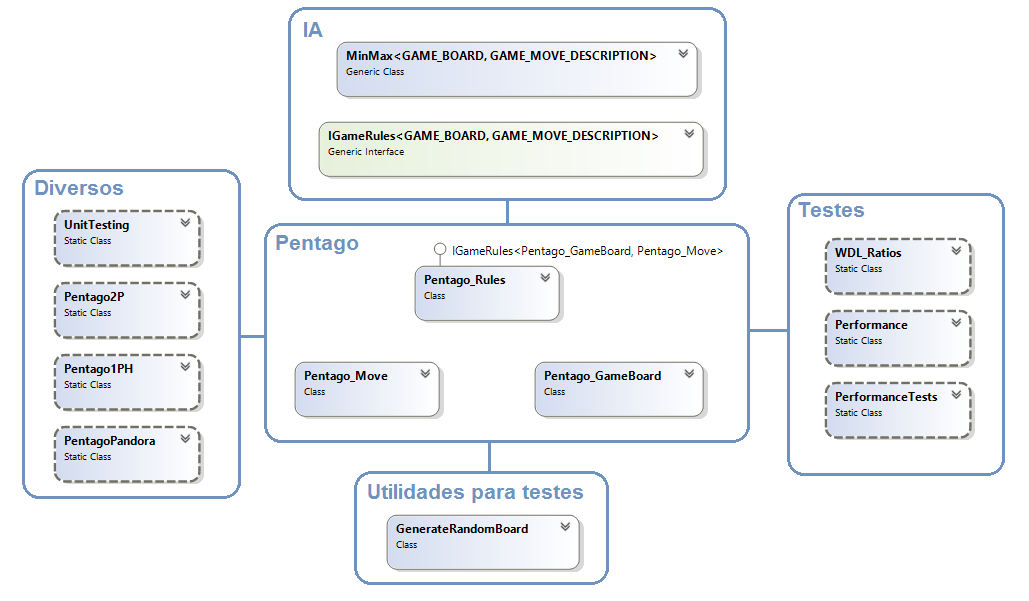
\includegraphics[height=8cm]{images/ClassDiagram1.png}
\end{table}


\newpage
\subsubsection{Descrição das Classes e Interfaces}

\begin{itemize}  

\item MinMax \\
Contem a implementação genérica do algoritmo de Minmax e variantes.

\item IGameRules \\
Interface necessária à implementação de um Minmax genérico, não dependente do jogo que analisa. Uma implementação da interface deve conter duas estruturas de dados diferentes, uma para representação do ambiente de jogo (tabuleiro no caso do Pentago) e outra para representação das jogadas a efetuar sobre este. A Interface pode ser consultada no anexo ~\ref{IGameRules}.

\item Pentago\_GameBoard \\
Contem o array que representa o tabuleiro. Contem também uma variável que indica o qual o jogador a jogar e ainda qual o estado da jogada (colocar peça ou rodar quadrante). Também contem métodos auxiliares para identificar fim de jogo, clonar tabuleiros, transformar índices do tabuleiro e coordenadas e virse-versa. A classe é necessária para fazer uso da interface implementada.

\item Pentago\_Move \\
Contem informação necessária para representar uma jogada. Havendo dois tipos de jogadas poderia alternativamente optar-se pela a criação de 2 subclasses, uma para cada tipo de jogada ao invés de guardar as duas numa mesma. A classe é necessária para fazer uso da interface implementada.

\item Pentago\_Rules \\
Classe que implementa a Interface IGameRules para o Pentago. Contem também as funções de heurística, métodos para identificação de simetrias e de tabuleiros idênticos. A classe é extensa e foi divida em vários ficheiros. Em conjunto com Pentago\_Move e Pentago\_GameBoard formam a implementação do jogo concreto.

\item GenerateRandomBoard \\
Como o nome sugere a classe é responsável pela geração de tabuleiros aleatórios que são usados nos testes de \verb|performance|. 

\item WDL\_Ratios \\
Responsável por testar a \verb|performance| das heurísticas e do Minmax em termos de taxa de vitórias, derrotas e empates e fazer output dos resultados já formatados para serem inseridos em Latex.

\item Performance \\
Classe que testa a \verb|performance| temporal de uma heurística para um dado conjunto de tabuleiros.

\item PerformanceTests \\
Classe responsável por testar a \verb|performance| temporal das várias heurísticas. 

\item PentagoPandora \\
\label{PandoraDescricao}
Classe cuja única função é descobrir e exportar para memória não volátil uma árvore de Minmax apenas para o primeiro jogador, com raiz no tabuleiro inicial, que permita garantir a vitória. Não tendo sido totalmente otimizada para efetuar o seu objetivo, acabou por ser deixada de lado uma vez que saia do âmbito do projeto.

\item Pentago2P \\
Classe que apenas implementa uma versão do Pentago para 2 jogadores em consola. Usada inicialmente para testar o código.

\item Pentago1PH \\
Apenas usada no inicio do desenvolvimento, antes de codificado o algoritmo de Minmax. Permitia a um jogador humano jogar contra um minmax com profundidade de 1 jogada.

\item UnitTesting \\
Classe com testes unitários. 

\end{itemize}
